\documentclass[a4paper,12pt]{article}

\usepackage[utf8x]{inputenc}
\usepackage[english, russian]{babel}

\usepackage{tabularx}
\usepackage{multirow}
\usepackage{graphicx}
\usepackage{misccorr}
\usepackage{indentfirst}
\usepackage{amsmath}


\usepackage{listings}
\usepackage{xcolor}

\usepackage{fullpage}

\usepackage[labelsep=endash,
		    margin=10pt, 
		    justification = centerlast, 
		    format = hang,
		    singlelinecheck=false
		    ]{caption}


\exhyphenpenalty=10000
\doublehyphendemerits=10000
\finalhyphendemerits=5000

\definecolor{codegreen}{rgb}{0,0.6,0}
\definecolor{codegray}{rgb}{0.5,0.5,0.5}
\definecolor{codepurple}{rgb}{0.58,0,0.82}
\definecolor{backcolour}{rgb}{0.95,0.95,0.92}
 
\lstdefinestyle{mystyle}{
    backgroundcolor=\color{backcolour},
    commentstyle=\color{codegreen},
    keywordstyle=\color{blue},
    numberstyle=\tiny\color{codegray},
    stringstyle=\color{codepurple},
    basicstyle=\footnotesize,
    breakatwhitespace=false,
    breaklines=true,
    captionpos=t,
    keepspaces=true,
    numbers=left,
    numbersep=5pt,
    showspaces=false,
    showstringspaces=false
    showtabs=false,
    tabsize=4,
    frame=tb
}
 
\lstset{style=mystyle}

\usepackage{color}
\usepackage{xcolor}
\usepackage{listings}
 
% Цвета для кода
 
\definecolor{string}{HTML}{B40000} % цвет строк в коде
\definecolor{comment}{HTML}{008000} % цвет комментариев в коде
\definecolor{keyword}{HTML}{1A00FF} % цвет ключевых слов в коде
\definecolor{morecomment}{HTML}{8000FF} % цвет include и других элементов в коде

\definecolor{сaptiontext}{HTML}{FFFFFF} % цвет текста заголовка в коде
\definecolor{сaptionbk}{HTML}{999999} % цвет фона заголовка в коде
\definecolor{bk}{HTML}{FFFFFF} % цвет фона в коде
\definecolor{frame}{HTML}{999999} % цвет рамки в коде
\definecolor{brackets}{HTML}{B40000} % цвет скобок в коде
 

%%% Отображение кода %%%
 
% Настройки отображения кода
 
\lstset{
	%morekeywords={*,...}, % если хотите добавить ключевые слова, то добавляйте	 
	% Настройки отображения     
	breaklines=true, % Перенос длинных строк
	% Для отображения русского языка
	extendedchars=true,
	literate={Ö}{{\"O}}1
	{Ä}{{\"A}}1
	{Ü}{{\"U}}1
	{ß}{{\ss}}1
	{ü}{{\"u}}1
	{ä}{{\"a}}1
	{ö}{{\"o}}1
	{~}{{\textasciitilde}}1
	{а}{{\selectfont\char224}}1
	{б}{{\selectfont\char225}}1
	{в}{{\selectfont\char226}}1
	{г}{{\selectfont\char227}}1
	{д}{{\selectfont\char228}}1
	{е}{{\selectfont\char229}}1
	{ё}{{\"e}}1
	{ж}{{\selectfont\char230}}1
	{з}{{\selectfont\char231}}1
	{и}{{\selectfont\char232}}
1
	{й}{{\selectfont\char233}}1
	{к}{{\selectfont\char234}}1
	{л}{{\selectfont\char235}}1
	{м}{{\selectfont\char236}}1
	{н}{{\selectfont\char237}}1
	{о}{{\selectfont\char238}}1
	{п}{{\selectfont\char239}}1
	{р}{{\selectfont\char240}}1
	{с}{{\selectfont\char241}}1
	{т}{{\selectfont\char242}}1
	{у}{{\selectfont\char243}}1
	{ф}{{\selectfont\char244}}1
	{х}{{\selectfont\char245}}1
	{ц}{{\selectfont\char246}}1
	{ч}{{\selectfont\char247}}1
	{ш}{{\selectfont\char248}}1
	{щ}{{\selectfont\char249}}1
	{ъ}{{\selectfont\char250}}1
	{ы}{{\selectfont\char251}}1
	{ь}{{\selectfont\char252}}1
	{э}{{\selectfont\char253}}1
	{ю}{{\selectfont\char254}}1
	{я}{{\selectfont\char255}}1
	{А}{{\selectfont\char192}}1
	{Б}{{\selectfont\char193}}1
	{В}{{\selectfont\char194}}1
	{Г}{{\selectfont\char195}}1
	{Д}{{\selectfont\char196}}1
	{Е}{{\selectfont\char197}}1
	{Ё}{{\"E}}1
	{Ж}{{\selectfont\char198}}1
	{З}{{\selectfont\char199}}1
	{И}{{\selectfont\char200}}1
	{Й}{{\selectfont\char201}}1
	{К}{{\selectfont\char202}}1
	{Л}{{\selectfont\char203}}1
	{М}{{\selectfont\char204}}1
	{Н}{{\selectfont\char205}}1
	{О}{{\selectfont\char206}}1
	{П}{{\selectfont\char207}}1
	{Р}{{\selectfont\char208}}1
	{С}{{\selectfont\char209}}1
	{Т}{{\selectfont\char210}}1
	{У}{{\selectfont\char211}}1
	{Ф}{{\selectfont\char212}}1
	{Х}{{\selectfont\char213}}1
	{Ц}{{\selectfont\char214}}1
	{Ч}{{\selectfont\char215}}1
	{Ш}{{\selectfont\char216}}1
	{Щ}{{\selectfont\char217}}1
	{Ъ}{{\selectfont\char218}}1
	{Ы}{{\selectfont\char219}}1
	{Ь}{{\selectfont\char220}}1
	{Э}{{\selectfont\char221}}1
	{Ю}{{\selectfont\char222}}1
	{Я}{{\selectfont\char223}}1
	{і}{{\selectfont\char105}}1
	{ї}{{\selectfont\char168}}1
	{є}{{\selectfont\char185}}1
	{ґ}{{\selectfont\char160}}1
	{І}{{\selectfont\char73}}1
	{Ї}{{\selectfont\char136}}1
	{Є}{{\selectfont\char153}}1
	{Ґ}{{\selectfont\char128}}1
	{\{}{{{\color{brackets}\{}}}1 % Цвет скобок {
	{\}}{{{\color{brackets}\}}}}1 % Цвет скобок }
}


\begin{document}

\begin{titlepage}
\newpage

\

\begin{center}
	\large		
   	Министерство образования и науки Российской Федерации\\[0.5cm]
    	
	ФГБОУ ВО Рыбинский государственный авиационный технический университет имени П.А. Соловьева\\[1.0cm]

	Факультет радиоэлектроники и информатики\\[0.25cm]
		
	Кафедра математического и программного обеспечения\\ электронных вычислительных средств\\[1.5cm]

	\Large
	\textbf{\textsc{ОТЧЕТ ПО ЛАБОРАТОРНОЙ РАБОТЕ}}\\[0.25cm]
	по  дисциплине\\
	\textbf{Математические методы анализа данных}\\[0.5cm]
	
	по теме\\
	
\end{center}

\vfill	
\begin{tabularx}{0.95\textwidth}{lXr}
Студент группы ИПБ-13 & &	Иванов Р.А.\\
Преподаватель, доцент & &	Воробьев К. А.
\end{tabularx}

\vfill 
\center Рыбинск 2017
\end{titlepage}	

\tableofcontents
\setcounter{page}{2}

\newpage\section{Гистограммы} 

Ниже представлена гистограмма для выборки, каждый элемент которой представляет среднее арифметическое выборки с равномерным распредилением объёмом 3 (рис.~\ref{fig:im_1}). Распределение имеет нормальный вид.
\begin{center}
	\begin{figure}[h]
	    \centering
   		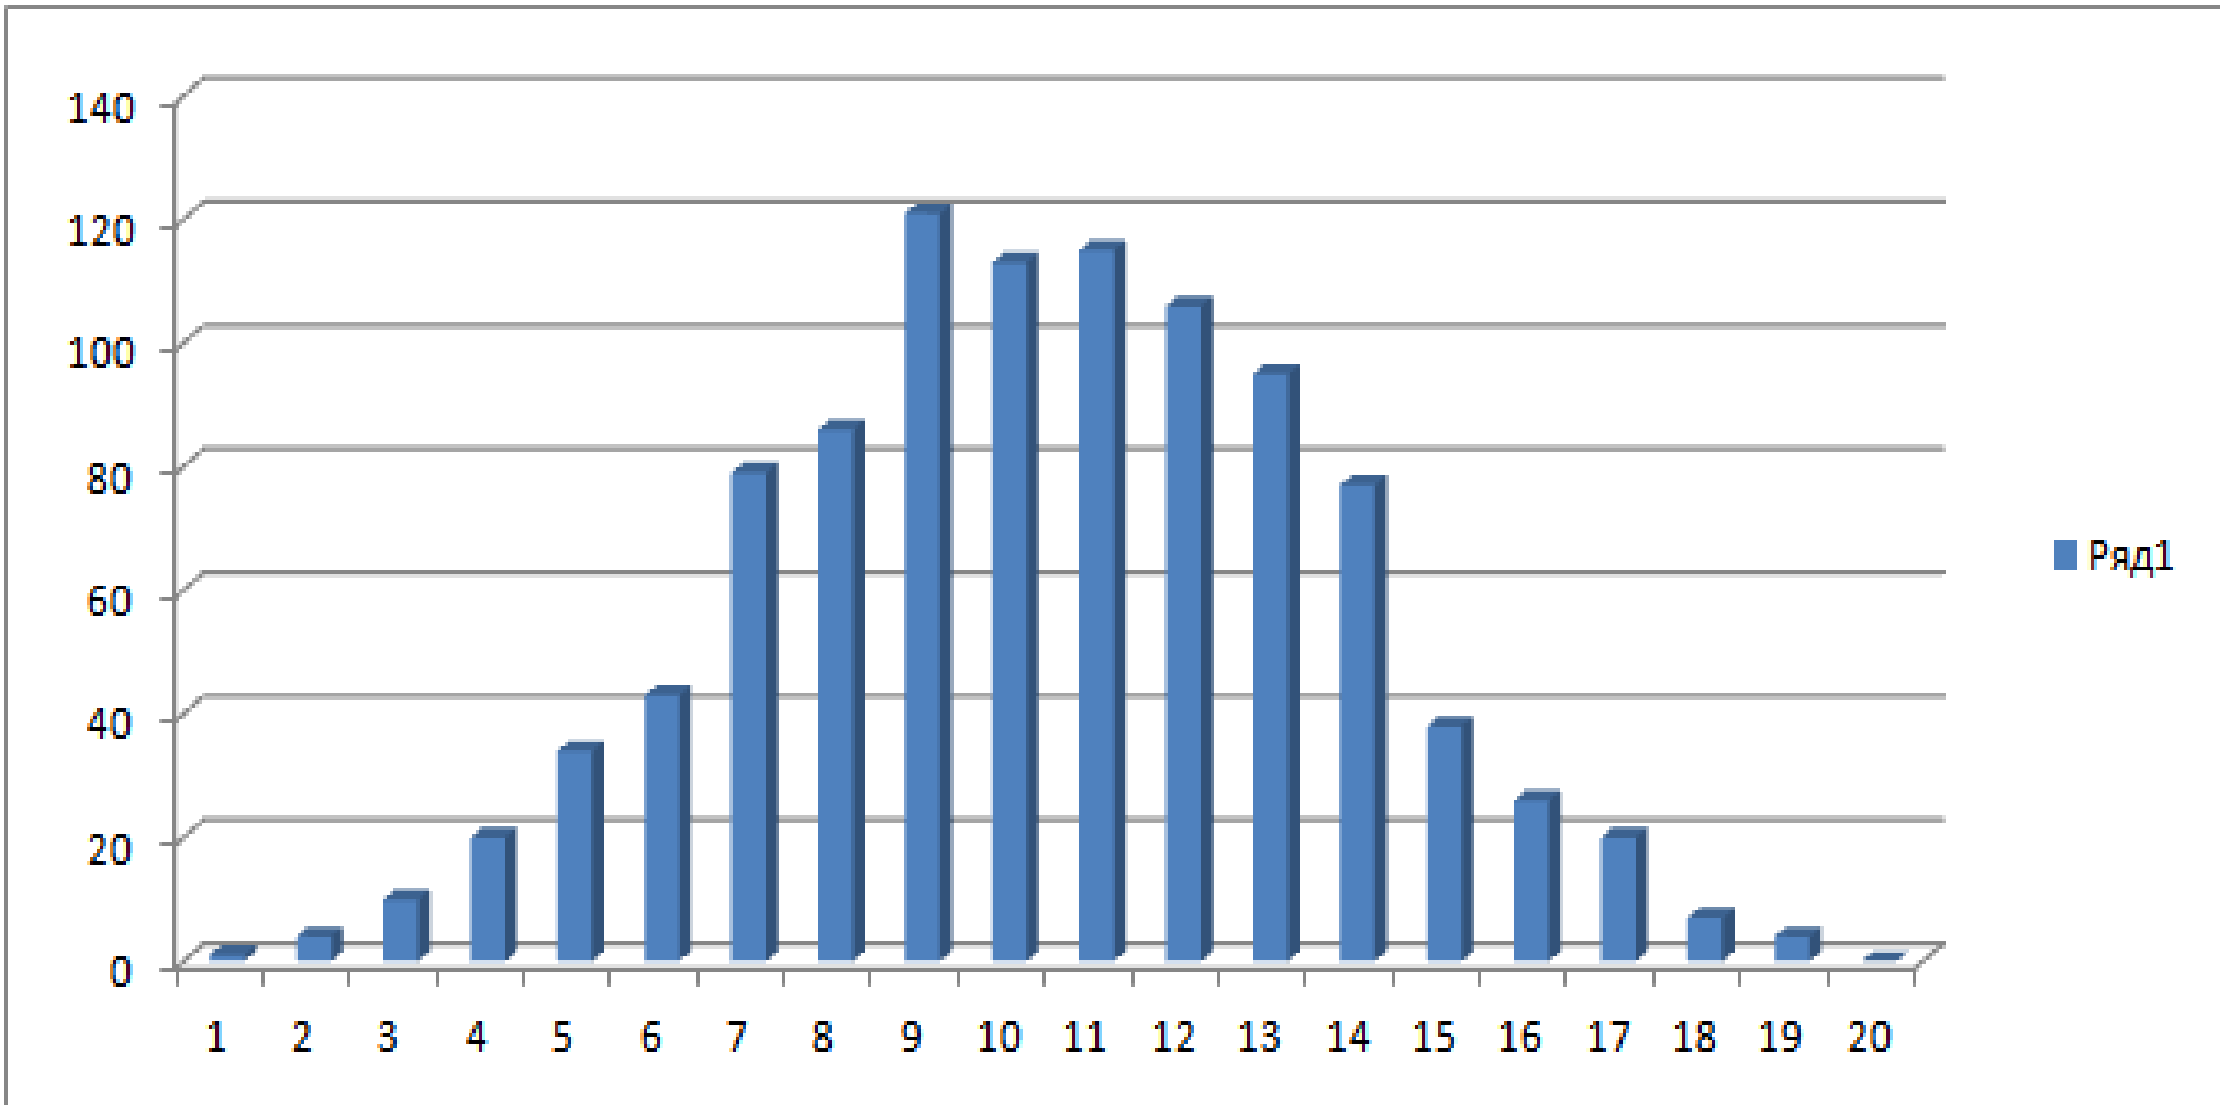
\includegraphics[scale=0.3]{figure_1.png}
   		\caption{Гистограмма для выборки из 3 элементов сложения}
   		\label{fig:im_1}
    \end{figure}
\end{center}
Хотя на графики видно, что распределение имеет нормальный вид, но нам бы хотелось более ярко выраженный "колокол".

\newpage
При выборке из 20 элементов сложения (рис.~\ref{fig:im_2}) видно, что среднее квадратичное отклонение стало меньше.
\begin{center}
	\begin{figure}[h]
		\centering
   		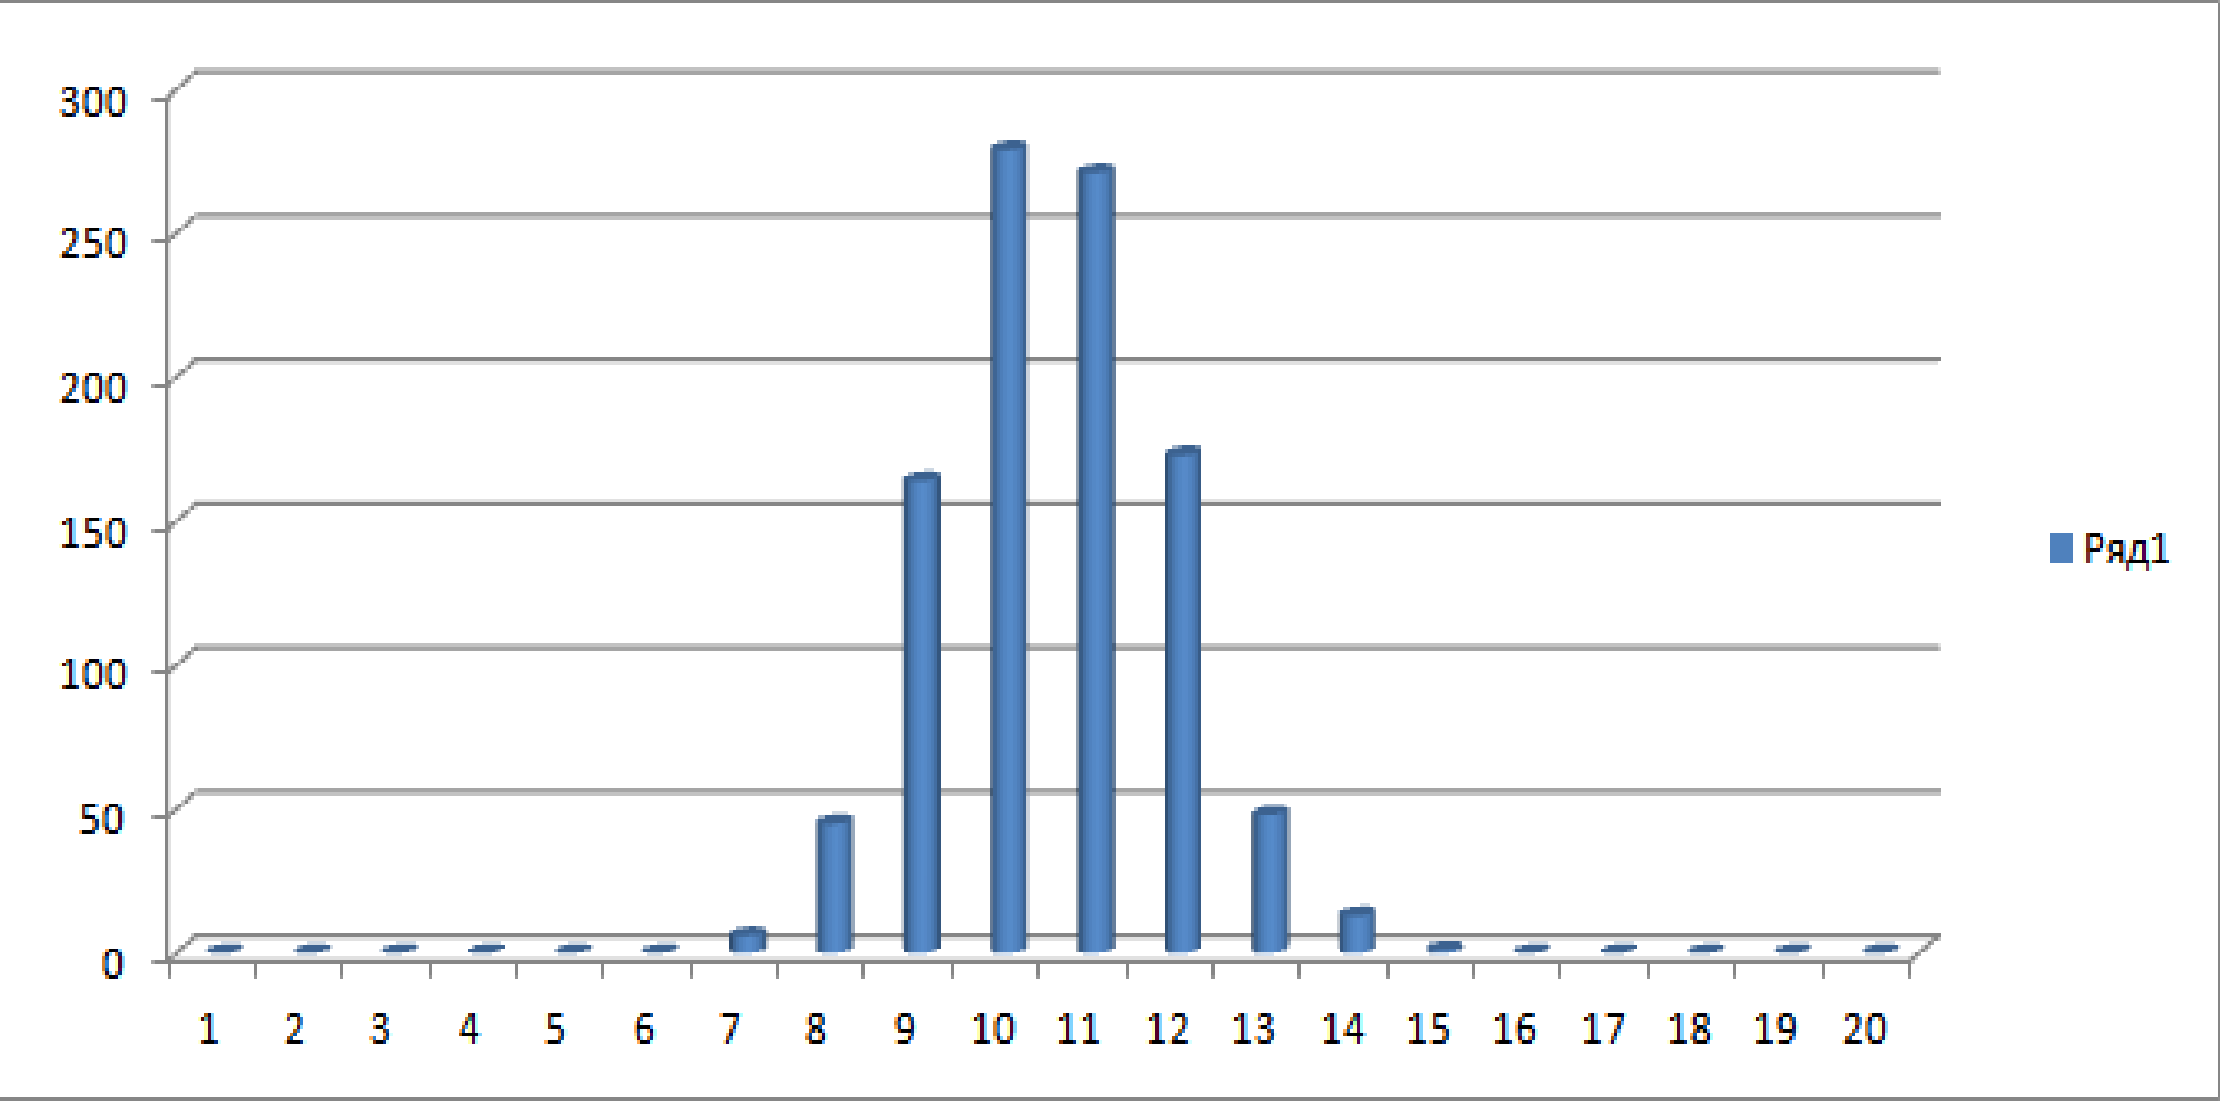
\includegraphics[scale=0.3]{figure_2.png}
   		\caption{Гистограмма для выборки из 20 элементов сложения}
   		\label{fig:im_2}
    \end{figure}
\end{center}
"Колокол" графика стал уже, но все еще оставляет желать лучшего, т. к. мы можем на нем видеть, что некторые столбцы чуть выше или чуть ниже. А значит нам нужно, по следствию из центральной предельной теоремы, увеличить число слагаемых.

\newpage
При выборке из 10 элементов сложения (рис.~\ref{fig:im_3}) видно, что "колокол" стал ещё выше и уже. Из центральной предельной теоремы следует, что среднее квадратичное отклонение этого распределения должно быть в 2 раза меньше, чем в предыдущего, что и видно на гистограмме.
\begin{center}
	\begin{figure}[h]
		\centering
   		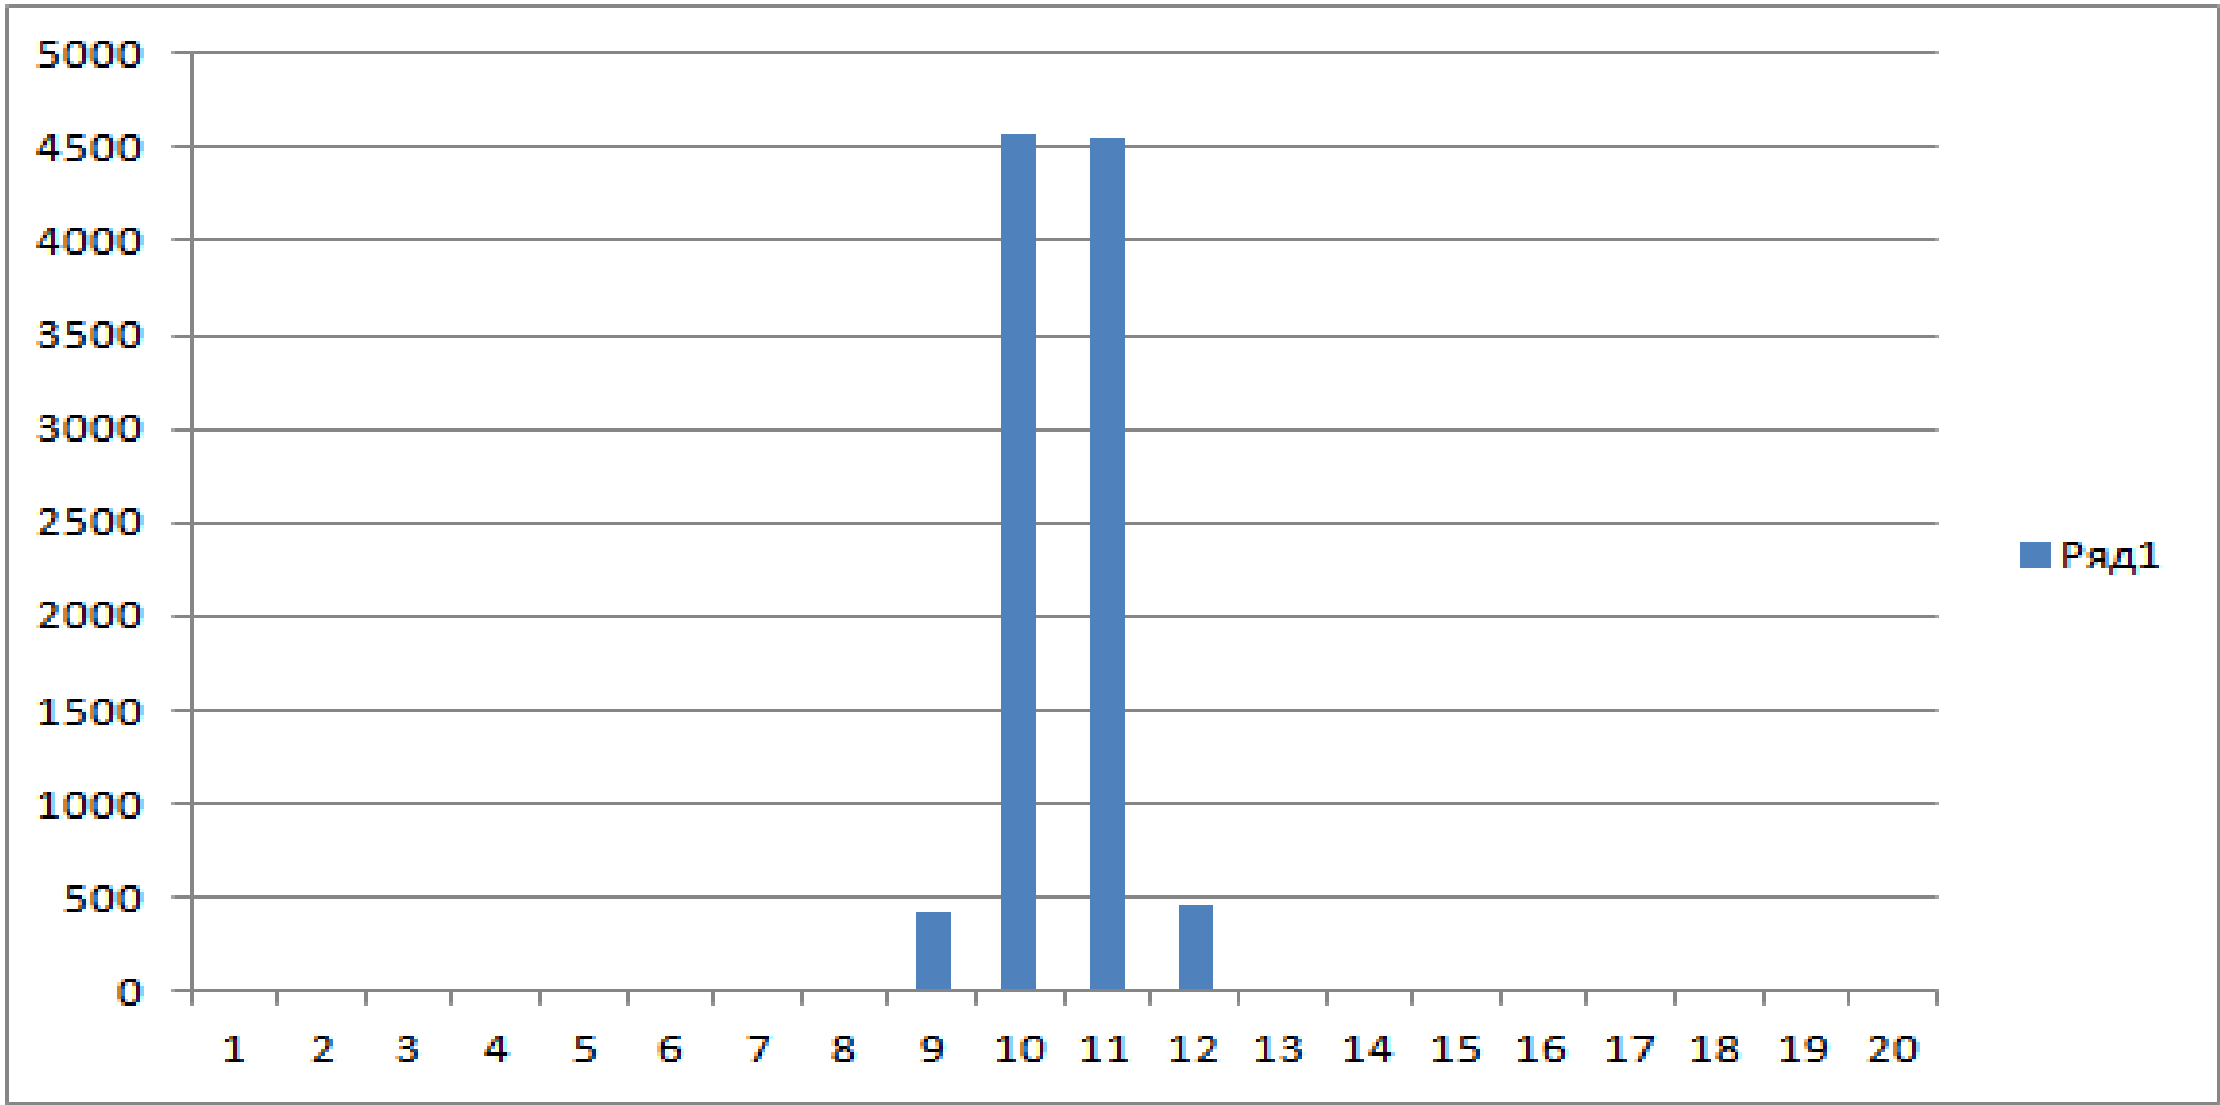
\includegraphics[scale=0.3]{figure_3.png}
   		\caption{Гистограмма для выборки из 100 элементов сложения}
   		\label{fig:im_3}
    \end{figure}
\end{center}

\newpage\section{Коэффициенты ковариации}

Ковариация – мера линейной зависимости двух случайных величин.

Знак коэффицента ковариации указывает на вид линейной связи между рассматриваемыми величинами: если он > 0 - это означает прямую связь (при росте одной величины растет и другая), < 0 указывает на обратную связь. При коэффициенте = 0 линейная связь между выборками при нулевом сдвиге отсутствует.

{\large $$cov(X, Y) = \frac{1}{n}\sum\limits_{i=1}^n x_i y_i - \left(\frac{1}{n}\sum\limits_{i=1}^n x_i \right) \left( \frac{1}{n} \sum\limits_{i=1}^n y_i \right)$$}

% $\fnum{-2.2986e-5}$

Ниже представлена ковариацилнная матрица для выборки из 100 элементов сложения.
{\tiny
$$
\begin{bmatrix}
7.912E-4 &3.47E-5 &-2.69E-5 &-8.33E-5 &1.5E-6 &-6.0E-5 &-1.82E-5 &5.4E-5 &2.29E-5 &2.26E-5 \\
3.47E-5 &7.808E-4 &-7.68E-5 &3.29E-5 &1.13E-5 &4.76E-5 &5.98E-5 &-2.8E-6 &-3.39E-5 &-2.81E-5 \\
-2.69E-5 &-7.68E-5 &9.15E-4 &7.1E-6 &-1.94E-5 &-1.15E-5 &-4.89E-5 &5.07E-5 &2.68E-5 &-4.6E-6 \\
-8.33E-5 &3.29E-5 &7.1E-6 &8.472E-4 &1.44E-5 &-3.52E-5 &-2.38E-5 &-1.1E-5 &-2.93E-5 &-9.9E-6 \\
1.5E-6 &1.13E-5 &-1.94E-5 &1.44E-5 &7.754E-4 &-6.49E-5 &2.88E-5 &5.0E-6 &-8.6E-6 &-6.9E-6 \\
-6.0E-5 &4.76E-5 &-1.15E-5 &-3.52E-5 &-6.49E-5 &9.101E-4 &4.35E-5 &-1.17E-5 &4.62E-5 &2.68E-5 \\
-1.82E-5 &5.98E-5 &-4.89E-5 &-2.38E-5 &2.88E-5 &4.35E-5 &9.212E-4 &-1.79E-5 &4.99E-5 &2.55E-5 \\
5.4E-5 &-2.8E-6 &5.07E-5 &-1.1E-5 &5.0E-6 &-1.17E-5 &-1.79E-5 &8.448E-4 &6.22E-5 &-4.34E-5 \\
2.29E-5 &-3.39E-5 &2.68E-5 &-2.93E-5 &-8.6E-6 &4.62E-5 &4.99E-5 &6.22E-5 &8.386E-4 &4.3E-6 \\
2.26E-5 &-2.81E-5 &-4.6E-6 &-9.9E-6 &-6.9E-6 &2.68E-5 &2.55E-5 &-4.34E-5 &4.3E-6 &8.227E-4 \\
\end{bmatrix} 
$$
}
Т.к. мы можем увидеть, что каждый элемент матрицы приближается к $0$ из этого делаем вывод, что переменные линейно независимы.


\newpage\section{Выборочные моменты}

В данном случае можно сказать, что начальным моментом $k$-го порядка случайной величины $X$ называется среднее арифметическое $k$-ой степени этой случайной величины.

{\large $$\alpha_k(X) = \sum\limits_{i=1}^n x_i^k p_i$$}

Центральным моментом $k$-го порядка случайной величины $X$ называется начальный момент $k$-ой степени отклонения случайной величины $X$ от её мат. ожидания.

{\large $$\mu_k(X) = \alpha_k\left(\left(X-M\left(X\right)\right)^k\right)$$}

Ввиду того, что все элементы выборки нормированны, теоретическое значение мат. ожидания составляет 0.5. Теоретическая дисперсия для каждой выборки исходя из свойств равномерно распределенной С.В. и центральной предельной теоремы составляет 0.02778, 0.0041667, 0.0008334 для выборок из 3, 20, 100 элементов сложения соответственно. Ниже представлены рассчетные значения моментов для каждой выборки ( таблицы~\ref{table:a_u_1}-\ref{table:a_u_3}). Можно заметить, что реальные значения дисперсии и мат. ожиданий близки к теоретическим значениям.

\begin{table}[h]
	\caption{Вычисленные моменты для выборки из 3 элементов сложения}
	\begin{tabular}{|c|c|c|}
	\hline 
	Порядок момента & Начальный момент & Центральный момент \\ 
	\hline 
	1 & 0.49638439340750873 & 4.951594689828198e-17 \\ 
	\hline 
	2 & 0.2722292309595661 & 0.0258317649410256\\ 
	\hline 
	3 & 0.16079444249574035 &  1.913087629077591e-05 \\ 
	\hline 
	4 & 0.10078517219460696 & 0.0018461873150255987 \\ 
	\hline 
	\end{tabular} 

	\label{table:a_u_1}
\end{table}

\begin{table}[h]
	\caption{Вычисленные моменты для выборки из 20 элементов сложения}
	\begin{tabular}{|c|c|c|}
	\hline 
	Порядок момента & Начальный момент & Центральный момент \\ 
	\hline 
	1 & 0.5017406913785922 & 2.2204460492503132e-17 \\ 
	\hline 
	2 & 0.255828559317913 & 0.00408483793284526 \\ 
	\hline 
	3 & 0.1324864894567112 & 2.783241296176622e-05 \\ 
	\hline 
	4 & 0.06964790298961453 &  4.71493015071018e-05 \\ 
	\hline 
	\end{tabular} 

	\label{table:a_u_2}
\end{table}

\begin{table}[h]
	\caption{Вычисленные моменты для выборки из 100 элементов сложения}
	\begin{tabular}{|c|c|c|}
	\hline 
	Порядок момента & Начальный момент & Центральный момент \\ 
	\hline 
	1 & 0.4992792925566728 & 9.270362255620058e-18 \\ 
	\hline 
	2 & 0.2500710439934647 & 0.000791232017573033 \\ 
	\hline 
	3 & 0.1256477706088138 &  2.3851508840121784e-06 \\ 
	\hline 
	4 &  0.0633305312395699 & 1.9141436304834823e-06 \\ 
	\hline 
	\end{tabular} 
	
	\label{table:a_u_3}
\end{table}

Так же мы можем заметить, что 3 центральный момент близок к $0$, из-за чего мы можем утвержать, что относительно мат. ожидание наши выборки симметричны.

\newpage\section{Доверительный интервал}
Доверительный интервал $(d)$ уровня $0.95$ определяет интервал, в который с вероятностью $95\%$ попадет мат. ожидание $(\alpha_1)$ элементов выборки.

{\large $$d=t\sqrt{\frac{m_2}{n}}$$}

Где $t$ в данном случае равно 1.96.

Во всех случая мат. ожидания находятся в пределах доверительных интервалов (таблица~\ref{table:d}).

\begin{table}[h]
	\caption{Вычисленные значения доверительных интервалов и мат. ожиданий}
	\begin{tabular}{|c|c|c|c|}
	\hline 
	Кол-во сложений & 0.5 - d & мат. ожидание($a_1$) & 0.5 + d \\ 
	\hline 
	3 & 0.490038308 & 0.49638439340750873 & 0.509961692 \\ 
	\hline 
	20 & 0.496038648 & 0.5017406913785922 & 0.503961352 \\ 
	\hline
	100 & 4.98e-01 & 0.4992792925566728 & 5,02e-01 \\ 
	\hline 
	\end{tabular}
	\label{table:d} 
\end{table}

\newpage\section{Общая оценка качества генератора}
При достаточно большом размерер выборки(эмперически установлено, что лучше брать выборки не меньше 10000 отсчётов), рассмотренный генератор случайных чисел на основе линейного конгруэнтного метода даёт распределение очень близкое к нормальному с характерестиками близкими к тем, которые следуют из центральной предельной теоремы. Мат. ожидания находятся в пределах доверительных интевалов с вероятностью 95\%. Достаточно низкий коэффициент ковариации говорит об отсутствии  линейной зависимости выборок с при нулевом сдвиге.

\newpage\section{Приложение}

\begin{lstlisting}[language=Java, title=Генератор случайных чисел из прошлой работы]

package ravnrasp;


/**
 * Клвсс для генерации рандомного числа
 * Created by Roman on 03.01.2017.
 */
public class Random {

    public static double a = 8121;
    public static double c = 28411;
    public static int m = 134456;
    public static double seed = 2;

    /**
     * Метод генерирует рандомное число от 0 до 1
     */
    public static double getRand() {
        seed = (a * seed + c) % m;
        return seed / (double) m;
    }

    /**
     * Генерирует рандомное число в диапазоне от a до b
     */
    public static double getRand(int a, int b) {
        return (double) a + ((double) b - (double) a) * getRand();
    }
}
\end{lstlisting}

\begin{lstlisting}[language=Java, title=Генератор случайных чисел]

package ravnrasp;

import java.util.ArrayList;

/**
 *
 * @author Roman
 */
public class RavnRandom {

    public static double ravnRandom(int k) {
        ArrayList<Double> array = new ArrayList<>();
        for (int i = 0; i < k; i++) {
            array.add(Random.getRand());
        }
        double result = array.stream()
                .reduce((s1, s2) -> s1 + s2)
                .orElse(0d);
        
        return result / k;
    }
}
\end{lstlisting}


\begin{lstlisting}[language=Java, title=Рассчет и отображение параметров распределения]

package ravnrasp;

import java.util.ArrayList;
import java.util.List;

import static java.util.stream.Collectors.toList;

/**
 * Класс для вспомогательных вычислений
 *
 * @author Roman
 */
public class CalculationHelper {

    /**
     * Расчитывает математическое ожидание случайной велечины
     *
     * @param list список случайных велечин
     * @return математическое ожидание
     */
    public static double calculateExpectedValue(List<Double> list) {
        double sum = list.stream()
                .mapToDouble(s -> s)
                .sum();
        return sum / list.size();
    }

    /**
     * Расчитать начальный момент случайной велечины
     *
     * @param list список случайныъ велечин
     * @param k степень
     * @return начальный момент
     */
    public static double calculateInitialMoment(List<Double> list, int k) {
        return calculateExpectedValue(list.stream()
                .map(s -> Math.pow(s, k))
                .collect(toList())
        );
    }

    /**
     * Метод для подсчета матрицы коварриации
     * @param arrays
     * @param n
     * @return
     */
    public static double[][]
    calculateCovarMatr(ArrayList<ArrayList<Double>> arrays,
     int n) {
        double[][] result = new double[n][n];
        for (int i = 0; i < n; i++) {
            List<Double> x = arrays.get(i);
            for (int j = 0; j < n; j++) {
                List<Double> y = arrays.get(j);
                ArrayList<Double> array = new ArrayList<>();
                for (int k = 0; k < arrays.get(i).size(); k++) {
                    array.add(x.get(k) * y.get(k));
                }
                result[i][j] = calculateExpectedValue(array)
                        - (calculateExpectedValue(x) *
                        calculateExpectedValue(y));
            }
        }
        return result;
    }

    /**
     * Расчитать центральный момент случайной велечины
     *
     * @param list спсок случайных велечин
     * @param k степень
     * @return центральный момент
     */
    public static double calculateCentralMoment(List<Double> 
    list, int k) {
        double expValue = calculateExpectedValue(list);
        return calculateExpectedValue(list.stream()
                .map(s -> Math.pow(s - expValue, k))
                .collect(toList())
        );
    }

    /**
     * Расчитать выборочную дисперсию случайной велечины
     *
     * @param list список случайных велечин
     * @return дисперсия
     */
    public static double calculateDispersion(List<Double> list) {
        return calculateCentralMoment(list, 2);
    }

    /**
     * Посчитать коэффициент автокорелляции
     *
     * @param list список случайных велечин
     * @param k шаг
     * @return коэффициент автокорелляции
     */
    public static double calculateAutocorrelation(List<Double> list, 
    int k) {
        List<Double> forCalculationList
                = list.stream()
                .map(s -> s -= 0.5)
                .collect(toList());
        // количество пар использованых для расчета
        int manyPairs = 0;Random.getRand()
        List<Double> resultList = new ArrayList<>();
        for (int i = 0; i < forCalculationList.size(); i++) {
            double mult = forCalculationList.get(i);
            if (i + k < forCalculationList.size()) {
                mult *= forCalculationList.get(i + k);
                manyPairs++;
                resultList.add(mult);
            }
        }

        for (int i = 0; i < resultList.size(); i++) {
            double res = resultList.get(i);
            resultList.set(i, res / manyPairs);
        }

        double sum = resultList.stream()
                .mapToDouble(s -> s)
                .sum();

        return sum / calculateDispersion(list);
    }

    public static double calculateConfidenceInterval(List<Double> 
    list, Double t) {
        return t * Math.sqrt(calculateDispersion(list) / list.size());
    }
}

\end{lstlisting}


\end{document}
